\begin{frame}
  \frametitle{Analyzing Probabilistic/Approximate VLSI Design}
  \begin{itemize}
    \item Partial design problem~\cite{Gitina2013} of probabilistic design
          \pause
          \begin{itemize}
            \item Synthesize black-box outputs $T$ to realize specification
                  \pause
            \item \alert{Constraints on inputs} to black boxes: $D_i \subseteq X \cup Y$
          \end{itemize}
  \end{itemize}
  \pause
  \begin{figure}
    \centering
    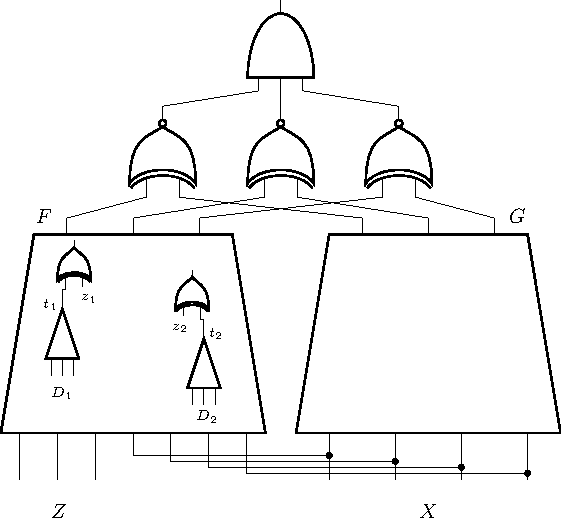
\includegraphics[scale=0.6]{fig/dssat-prob-miter.pdf}
  \end{figure}
  \pause
  \begin{align*}
    \random{} X,\random{} Z,\forall Y,\exists T(D).
    (Y \equiv E(X)) \limply (F(X,Z,T) \equiv G(X))
  \end{align*}
\end{frame}